\documentclass{article}
\usepackage[utf8]{inputenc}
\usepackage[greek,english]{babel}
\usepackage{alphabeta}
\usepackage{fancyhdr}
\usepackage{listings}
\usepackage{mathtools}
\usepackage{graphicx}
\usepackage{blindtext}
\usepackage{xcolor}
\usepackage{float}
\usepackage[backend=biber]{biblatex}

\title{Σήματα και Συστήματα - Εργασία 1}
\author{Χρήστος Μαργιώλης - 19390133}
\date{Μάρτιος 2021}

% uniwa logo

\begin{document}

\begin{titlepage}
        \maketitle
\end{titlepage}

\renewcommand{\contentsname}{Περιεχόμενα}
\tableofcontents

\section{'Ασκηση 1}

\begin{itemize}
        \item Δημιουργήστε ένα διάνυσμα $a = [0,0.1,0.2,...,10]$ και ένα διάνυσμα
                $b = [\cos(0),\cos(0.2),\cos(0.4),...,\cos(20)]$
        \item Να βρεθούν τα:
        \begin{itemize}
                \item $c = a / b$
                \item $d = a^4$
                \item το εσωτερικό γινόμενο των $a$ και $b$.
        \end{itemize}
\end{itemize}

Για να δημιουργήσουμε ένα διάνυσμα, τού δίνουμε ένα όνομα και στην συνέχεια μέσα
σε [] ορίζουμε τα στοιχεία χωρισμένα είτε με κόμμα είτε με κενά. Το διάνυσμα
που ζητείται από την εκφώνηση έχει την μορφή $0,0.1,0.2...,10$ το οποίο σημαίνει
ότι είναι ένα διάνυσμα με αριθμούς από το 1 έως το 10 με διάστηματα 0.1. Για να
αναπαραστήσουμε κάτι τέτοιο αυτόματα χωρίς να γράψουμε όλους τους αριθμούς μηχανικά,
δηλώνουμε το διάνυσμα ως εξής: αρχή:διάστημα:τέλος. Οπότε:

\begin{lstlisting}[language=octave]
        octave:1> a = 0:0.1:10
\end{lstlisting}

Αντίστοιχα για το διάνυσμα $b$, βλέπουμε ότι τα διαστήματα είναι $0.2$
και σε κάθε αριθμό του διανύσματος υπολογίζεται το συνημίτονο. Θα ορίσουμε
ένα διάνυσμα από το 0 έως το 20 με διαστήματα $0.2$ και θα υπολογίσουμε
τα συνημίτονα όλων των στοιχείων χρησιμοποιώντας την συνάρτηση \lstinline{cos()}:

\begin{lstlisting}[language=octave]
        octave:2> b = cos(0:0.2:20)
\end{lstlisting}

Για την διαίρεση διανυσμάτων χρησιμοποιούμε το σύμβολο / που χρησιμοποιείται
γενικότερα για διαίρεση, οπότε το $c = a / b$ θα γίνει:

\begin{lstlisting}[language=octave]
        octave:3> c = a / b
        c = 0.89415
\end{lstlisting}

Προκειμένου να υψώσουμε σε δύναμη όλα τα στοιχεία ενός διανύσματος πρέπει να
χρησιμοποιήσουμε τον τελεστή \lstinline{.^}, οπότε η πράξη $d = a^4$ θα γραφτεί
ως \lstinline{d = a.^4}. Αυτό το statement θα υπολογίσει ουσιαστικά την σειρά
\[d = [a_1^4, a_2^4, a_3^4, ..., a_n^4]\]
Η στοίχηση της εξόδου από το Octave έχει τροποποιηθεί
επειδή είναι πολύ μεγάλη και δεν χωράει σωστά στην σελίδα:

\begin{lstlisting}[language=octave]
        octave:4> d = a.^4
\end{lstlisting}
\begin{lstlisting}[language=octave,basicstyle=\tiny]
        d =

 Columns 1 through 17:

0.00000  0.00010   0.00160  0.00810  0.02560  0.06250  0.12960  0.24010 
0.40960  0.65610   1.00000  1.46410  2.07360  2.85610  3.84160  5.06250  6.55360

 Columns 18 through 34:

8.35210   10.49760  13.03210  16.00000  19.44810  23.42560  27.98410  33.17760
39.06250  45.69760  53.14410  61.46560  70.72810  81.00000  92.35210  104.85760  118.59210

 Columns 35 through 51:

133.63360  150.06250  167.96160  187.41610  208.51360  231.34410  256.00000
282.57610  311.16960  341.88010  374.80960  410.06250  447.74560  487.96810
530.84160  576.48010  625.00000

 Columns 52 through 68:

676.52010   731.16160   789.04810   850.30560   915.06250   983.44960   1055.60010
1131.64960  1211.73610  1296.00000  1384.58410  1477.63360  1575.29610  1677.72160
1785.06250  1897.47360  2015.11210

 Columns 69 through 85:

2138.13760  2266.71210  2401.00000  2541.16810  2687.38560  2839.82410
2998.65760  3164.06250  3336.21760  3515.30410  3701.50560  3895.00810
4096.00000  4304.67210  4521.21760  4745.83210  4978.71360

 Columns 86 through 101:

5220.06250  5470.08160  5728.97610  5996.95360  6274.22410  6561.00000
6857.49610  7163.92960  7480.52010  7807.48960  8145.06250  8493.46560
8852.92810  9223.68160  9605.96010  10000.00000
\end{lstlisting}

Για να υπολογίσουμε το εσωτερικό γινόμενο του $a$ και $b$, θα χρησιμοποιήσουμε
την συνάρτηση \lstinline{dot()} (Dot Product). Η συνάρτηση αυτή όταν εφαρμοστεί
στα διανύσματα $a$ και $b$, θα υπολογίσει την παρακάτω παράσταση:

\[x = a_1 \cdot b_1 + a_2 \cdot b_2 + a_3 \cdot b_3 + ... + a_n \cdot b_n\]

Οπότε:

\begin{lstlisting}[language=octave]
        octave:5> dot(a, b)
        ans = 46.051
\end{lstlisting}

\section{'Ασκηση 2}

\begin{itemize}
        \item Να γραφεί συνάρτηση (function) η οποία θα παίρνει ως όρισμα
                έναν αριθμό σε ακτίνια (rad) και θα επιστρέφει την τιμή του
                σε μοίρες.
        \item Βρείτε πόσες μοίρες είναι τα $\pi/4$ rad.
\end{itemize}

Για να δηλώσουμε μία συνάρτηση χρησιμοποιούμε την εντολή \lstinline{function}
ακολουθώμενη από από το όνομα της συνάρτησης. Εάν θέλουμε η συνάρτηση να δέχεται
ορίσματα, τα δηλώνουμε σε παρένθεση μετά το όνομα της συνάρτησης. Στην περίπτωση
που θέλουμε να επιστρέφεται και κάποια τιμή, δηλώνουμε το όνομά της μεταβλητής
που επιστρέφεται πριν το όνομα της συνάρτησης. Τέλος, για να σημάνουμε το τέλος
της συνάρτησης, γράφουμε την εντολή \lstinline{endfunction}

Για την συνάρτηση μετατροπής ακτινίων σε μοίρες θα χρειαστεί να υλοποιήσουμε
τον τύπο:
\[deg = rad \cdot 180 / \pi\]
Οπότε βάσει τα παραπάνω, η συνάρτηση θα υλοποιηθεί ως εξής:

\begin{lstlisting}[language=octave]
        function ret = deg(rad)
                ret = rad * 180 / pi
        endfunction
\end{lstlisting}

Τώρα μπορούμε να καλέσουμε την συνάρτηση δίνοντας της μία τιμή σε ακτίνια.
Τα $\pi / 4$ ακτίνια σε μοίρες είναι:

\begin{lstlisting}[language=octave]
        octave:6> x = deg(pi / 4)
        x = 45
\end{lstlisting}

\section{'Ασκηση 3}

\begin{itemize}
        \item Να γραφεί συνάρτηση (function) που να σχεδιάζει τη
                συνάρτηση: \[\sin c(x) = \frac{\sin(\pi x)}{\pi x}\]
        \item Σχεδιάστε τη για το διάστημα $[-2\pi,2\pi]$.
\end{itemize}

Για να σχεδιάσουμε την συνάρτηση 
\[\sin c(x) = \frac{\sin(\pi x)}{\pi x}, -2\pi < x < 2\pi\]
πρέπει να ακολουθήσουμε τα εξής βήματα στο Octave:

\begin{itemize}
        \item Να ορίσουμε το διάστημα $[-2\pi, 2\pi]$
        \item Να υπολογίσουμε το $c(x)$ για κάθε $x$
        \item Να υπολογίσουμε το $\sin c(x)$
\end{itemize}

Αρχικά, θα δηλώσουμε το διάστημα $[-2\pi,2\pi]$ με αποστάσεις 0.1
από τον κάθε αριθμό ώστε να έχουμε μία πιο ακριβή γραφική παράσταση.
Το διάνυσμα που θα προκύψει το αποθηκεύουμε στην μεταβλητή $x$:

\begin{lstlisting}[language=octave]
        octave:7> x = -2*pi:0.1:2*pi
\end{lstlisting}

'Επειτα υπολογίζουμε την συνάρτηση 
\[c(x) = \frac{\sin(\pi x)}{\pi x}\]
Είναι σημαντικό να σημειωθεί ότι
πρέπει να χρησιμοποιηθεί ο τελεστής ./ ώστε να επιστραφεί διάνυσμα
και όχι ένας αριθμός:

\begin{lstlisting}[language=octave]
        octave:8> c = sin(x * pi) ./ (pi * x)
\end{lstlisting}

Θα υπολογίσουμε το ημίτονο της συνάρτησης $c(x)$ κατευθείαν στην κλήση
της συνάρτησης σχεδίασης - η συναρτήση αυτή είναι η \lstinline{plot()} και παίρνει
ως ορίσματα τις τιμές του άξονα $x$ και $y$ (\lstinline{plot(x, y)}). Στην
προκειμένη περίπτωση θα της δώσουμε ως $x$ το $x$ που υπολογίσαμε στην αρχή,
και ως $y$ το συνημίτονο της συνάρτησης $c(x)$:

\begin{lstlisting}[language=octave]
        octave:9> plot(x, sin(c))
\end{lstlisting}

Παρατηρούμε ότι η γραφική παράσταση που προκύπτει έχει ένα \textit{ενδιαφέρον}
σχήμα:

\begin{figure}[H]
        \centering
        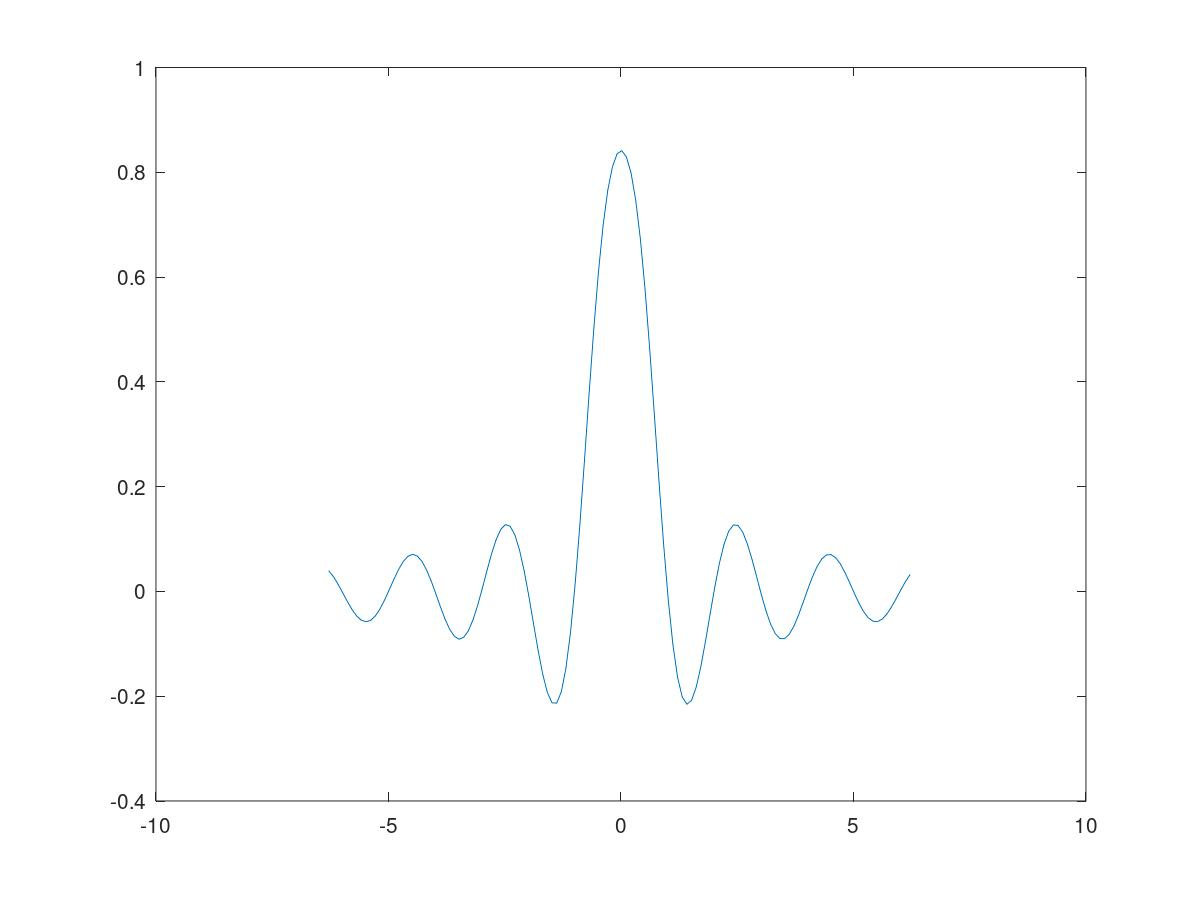
\includegraphics[width=\linewidth]{res/fig1.jpg}
        \caption{$\sin c(x) = \frac{\sin(\pi x)}{\pi x}, -2\pi < x < 2\pi$}
\end{figure}

\section{'Ασκηση 4}

\begin{itemize}
        \item Να γραφεί συνάρτηση (function) η οποία θα παίρνει ως όρισμα
        έναν μιγαδικό αριθμό και θα επιστρέφει:
        \begin{itemize}
                \item Την φάση.
                \item Το μέτρο.
                \item Το πραγματικό μέρος.
                \item Το φανταστικό μέρος του μιγαδικού.
        \end{itemize}
        \item Υπολογίστε τα παραπάνω μεγέθη για τους εξής μιγαδικούς:
        \begin{itemize}
                \item $i$
                \item $-i$
                \item $1$
                \item $e^{3+4i}$
        \end{itemize}
\end{itemize}

Το Octave (και το Matlab) διαθέτουν συναρτήσεις χειρισμού μιγαδικών αριθμών.

Για τον υπολογισμό της φάσης ενός μιγαδικού αριθμού χρησιμοποιούμε την συνάρτηση
\lstinline{angle()}. Η συνάρτηση αυτή όταν της δωθεί μιγαδικός αριθμός θα
υπολογίσει τον παρακάτω τύπο:
\[\theta = atan(y, x)\]

Ο υπολογισμός του μέτρου ενός μιγαδικού αριθμό γίνεται μέσω της συνάρτησης
\lstinline{abs()} η οποία εφαρμόζει τον παρακάτω τύπο:
\[|z| = \sqrt{x^2 + y^2}\]

Οι συναρτήσεις \lstinline{real()} και \lstinline{imag()} επιστρέφουν το πραγματικό
και φανταστικό αντίστοιχα μέρος ενός μιγαδικού αριθμού.

Οπότε με την χρήση όλων των παραπάνω συναρτήσεων μπορούμε να υλοποιήσουμε μία
συνάρτηση η οποία υπολογίζει και επιστρέφει κατευθείαν τις τέσσερεις αυτές
τιμές (φάση, μέτρο, πραγματικό μέρος, φανταστικό μέρος):

\begin{lstlisting}[language=octave]
        function imaginary(num)
                phase = angle(num)
                magnitude = abs(num)
                realpart = real(num)
                imagpart = imag(num)
        endfunction
\end{lstlisting}

Τώρα μπορούμε να δώσουμε στην συνάρτηση οποιοδήποτε μιγαδικό αριθμό για
επαληθεύσουμε ότι λειτουργεί σωστά.

Για $i$:
\begin{lstlisting}[language=octave]
        octave:10> imaginary(i)
        phase     =  1.5708
        magnitude =  1
        realpart  =  0
        imagpart  =  1
\end{lstlisting}

Για $-i$:
\begin{lstlisting}[language=octave]
        octave:11> imaginary(-i)
        phase     = -1.5708
        magnitude =  1
        realpart  = -0
        imagpart  = -1
\end{lstlisting}

Για $1$:
\begin{lstlisting}[language=octave]
        octave:12> imaginary(1)
        phase     = 0
        magnitude = 1
        realpart  = 1
        imagpart  = 0
\end{lstlisting}

Για $e^{3 + 4i}$:
\begin{lstlisting}[language=octave]
        octave:13> imaginary(e^(3 + 4*i))
        phase     = -2.2832
        magnitude =  20.086
        realpart  = -13.129
        imagpart  = -15.201
\end{lstlisting}

\section{'Ασκηση 5}

\begin{itemize}
        \item Διαχωρίστε το διάστημα $[0, 2\pi]$ σε 500 σημεία.
        \item Να σχεδιάσετε σε αυτό το διάστημα (στο ίδιο figure)
                τα παρακάτω σήματα:
        \begin{itemize}
                \item $f(x) = xe^{-x}, 0 < x < 2\pi$
                \item $y(x) = 2^{cos(x)}, 0 < x < 2\pi$
        \end{itemize}
        \item Βάλτε τίτλο στην γραφική παράσταση (ό,τι θέλετε).
        \item Βάλτε ταμπέλες στον $x$ και $y$ άξονα (ό,τι θέλετε).
        \item Βάλτε μία επιγραφή για όλες τις καμπύλες με την εντολή
                \lstinline{legend}.
        \item Να σχεδιάσετε τα δύο παραπάνω σήματα σε ένα δεύτερο figure
                αλλά σε \textbf{2 διαφορετικά} παράθυρα.
\end{itemize}

Για να χωρίσουμε το διάστημα $[0,2\pi]$, απλώς θα διαιρέσουμε το $2\pi$ με
500 ώστε να μας δώσει τις αποστάσεις ανάμεσα στους αριθμούς του διαστήματος.
Το διάνυσμα που θα φτιάξουμε εννοείται ότι θα το χρησιμοποιήσουμε ως $x$.

\begin{lstlisting}[language=octave]
        octave:14> 2 * pi / 500
        ans = 0.012566
\end{lstlisting}

Με αυτό το 0.012566 θα φτιάξουμε το διάνυσμα $x$:

\begin{lstlisting}[language=octave]
        octave:15> 0:0.012566:2*pi
\end{lstlisting}

Τώρα μπορούμε να υπολογίσουμε τα $f(x)$ και $y(x)$. Με παρόμοια λογική όπως
και στην προηγούμενη άσκηση, πρέπει να χρησιμοποιηθεί ο τελεστής \lstinline{.^}
και \lstinline{.*} ώστε να πάρουμε διάνυσμα και όχι αριθμό:

\begin{lstlisting}[language=octave]
        octave:16> f = x.*e.^-x
        octave:17> y = 2.^cos(x)
\end{lstlisting}

Σχεδιάζουμε την γραφική παράσταση της $f(x)$:

\begin{lstlisting}[language=octave]
        octave:18> plot(x, f)
\end{lstlisting}

Τώρα προκειμένου να σχεδιάσουμε και την γραφική παράσταση της $y(x)$ στο ίδιο
figure πρέπει να δώσουμε στο Octave την εντολή \lstinline{hold on} ώστε να μην
δημιουργήσει νέο παράθυρο για την $y(x)$. Στην συνέχεια σχεδιάζουμε και την $y(x)$:

\begin{lstlisting}[language=octave]
        octave:19> hold on
        octave:20> plot(x, y)
\end{lstlisting}

Σε αυτό το σημείο έχουνε σχεδιαστεί και οι δύο γραφικές παραστάσεις στο ίδιο figure.

\begin{figure}[H]
        \centering
        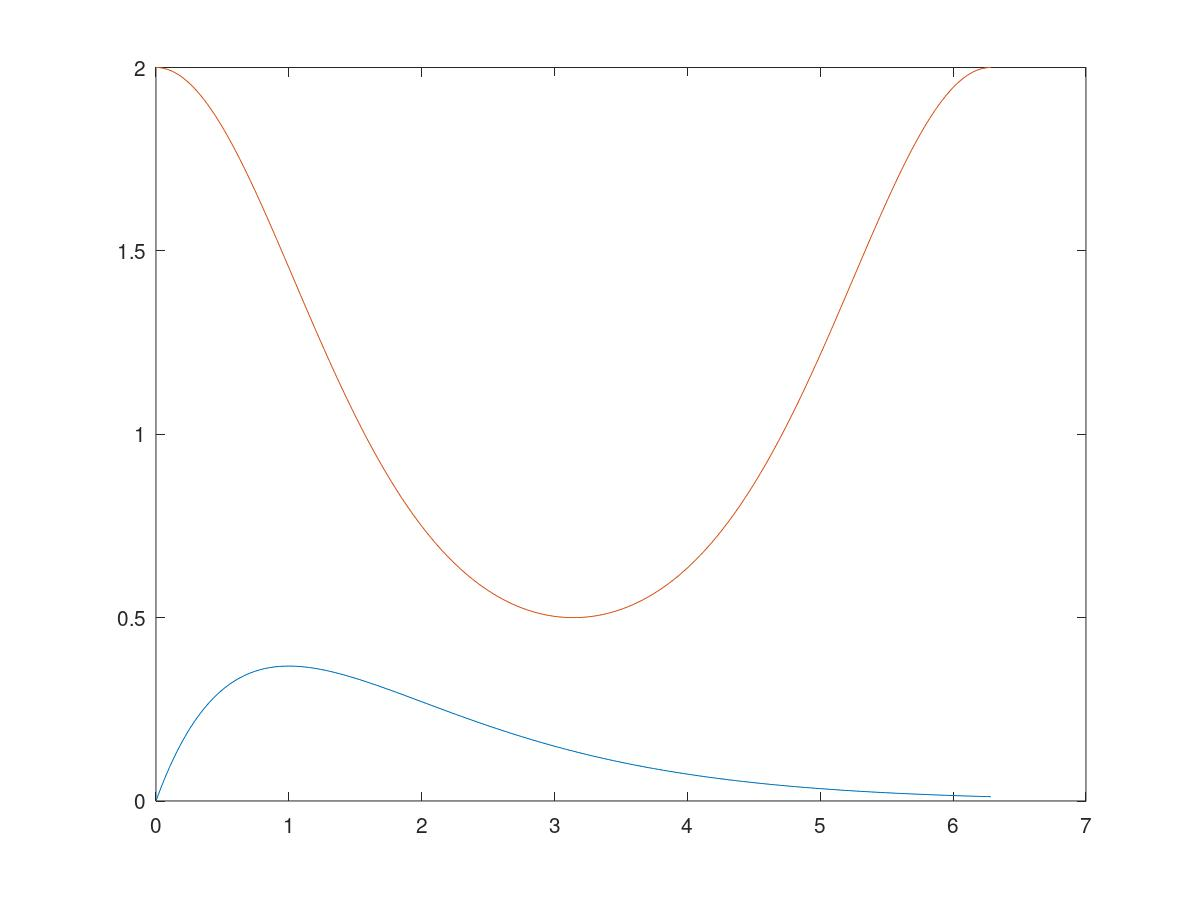
\includegraphics[width=\linewidth]{res/fig2.jpg}
        \caption{Μμπλε: $f(x) = xe^{-x}$, Πορτοκαλί: $y(x) = xe^{-x}$}
\end{figure}

Για να δώσουμε τίτλο στην γραφική παράσταση, χρησιμοποιούμε την συνάρτηση
\lstinline{title()} και σαν όρισμα της δίνουμε ένα string με τον τίτλο που θέλουμε.

\begin{lstlisting}[language=octave]
        octave:21> title("f(x) and y(x)")
\end{lstlisting}

Για τις ταμπέλες (labels) χρησιμοποιούμε τις συναρτήσεις \lstinline{xlabel()}
και \lstinline{ylabel()} για τους άξονες $x$ και $y$ αντίστοιχα. Σαν όρισμα δέχονται
ένα string με τις ταμπέλες που θέλουμε:

\begin{lstlisting}[language=octave]
        octave:22> xlabel("x")
        octave:23> ylabel("y")
\end{lstlisting}

Για να δώσουμε μία επιγραφή καλούμε την συνάρτηση \lstinline{legend()}.
Εφόσον θέλουμε το legend να περιέχει επιγραφή και για τις δύο συνάρτησεις
που σχεδιάσαμε, θα δώσουμε ως όρισμα στην \lstinline{legend()} τις επιγραφές
κλεισμένες σε αγκύλες και χωρισμένες με κόμμα:

\begin{lstlisting}[language=octave]
        octave:24> legend({"f(x)", "y(x)"})
\end{lstlisting}

\begin{figure}[H]
        \centering
        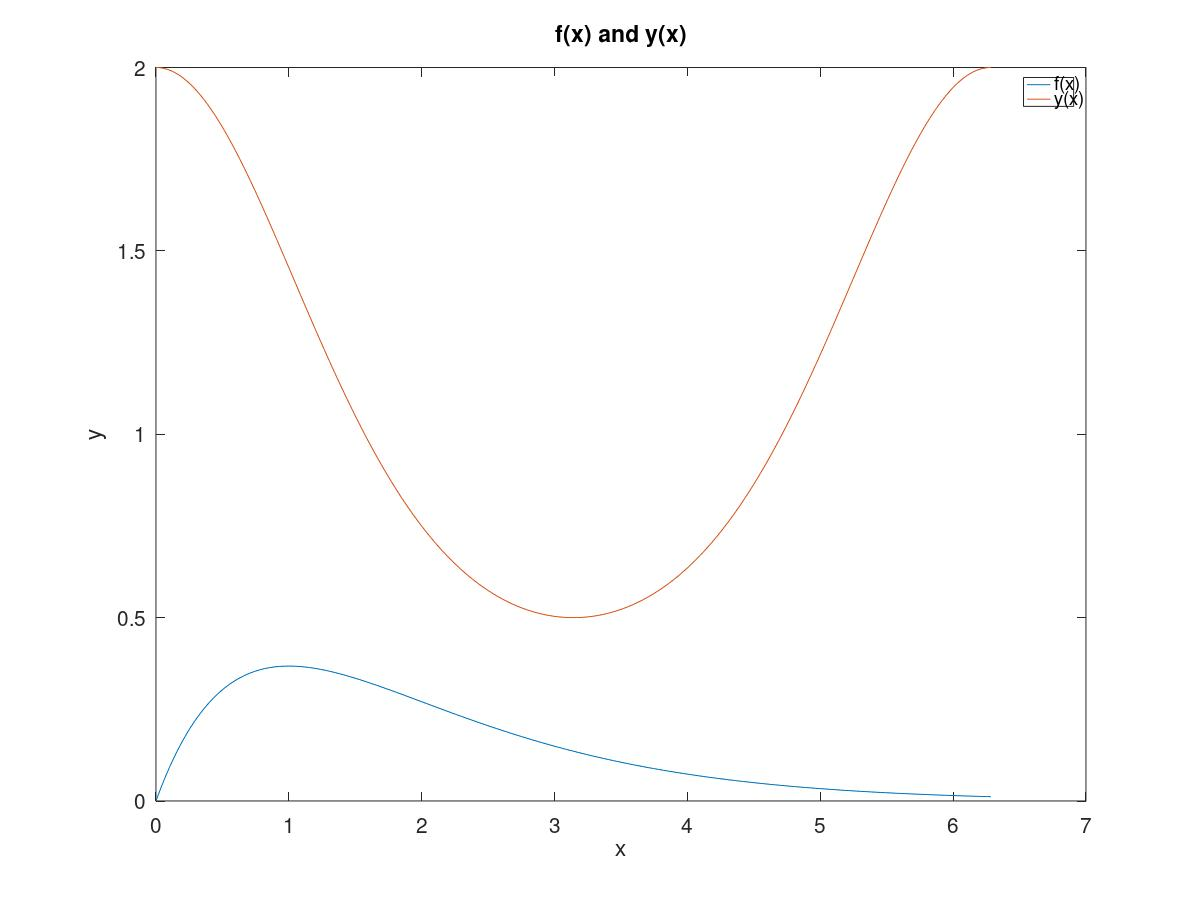
\includegraphics[width=\linewidth]{res/fig3.jpg}
        \caption{$f(x)$ και $y(x)$ με επιγραφές και τίτλο}
\end{figure}

Για να σχεδιάσουμε σε ξεχωριστά παράθυρα τις συναρτήσεις $f(x)$ και $y(x)$
θα ακολουθήσουμε την ίδια διακασία με πριν, αλλά χωρίς την εντολή
\lstinline{hold on}. Δηλαδή απλώς θα καλέσουμε δύο φορές την
\lstinline{plot()} - μία με όρισμα την $f(x)$ και μία με την $y(x)$.

\begin{lstlisting}[language=octave]
        octave:25> plot(x, f)
\end{lstlisting}

\begin{figure}[H]
        \centering
        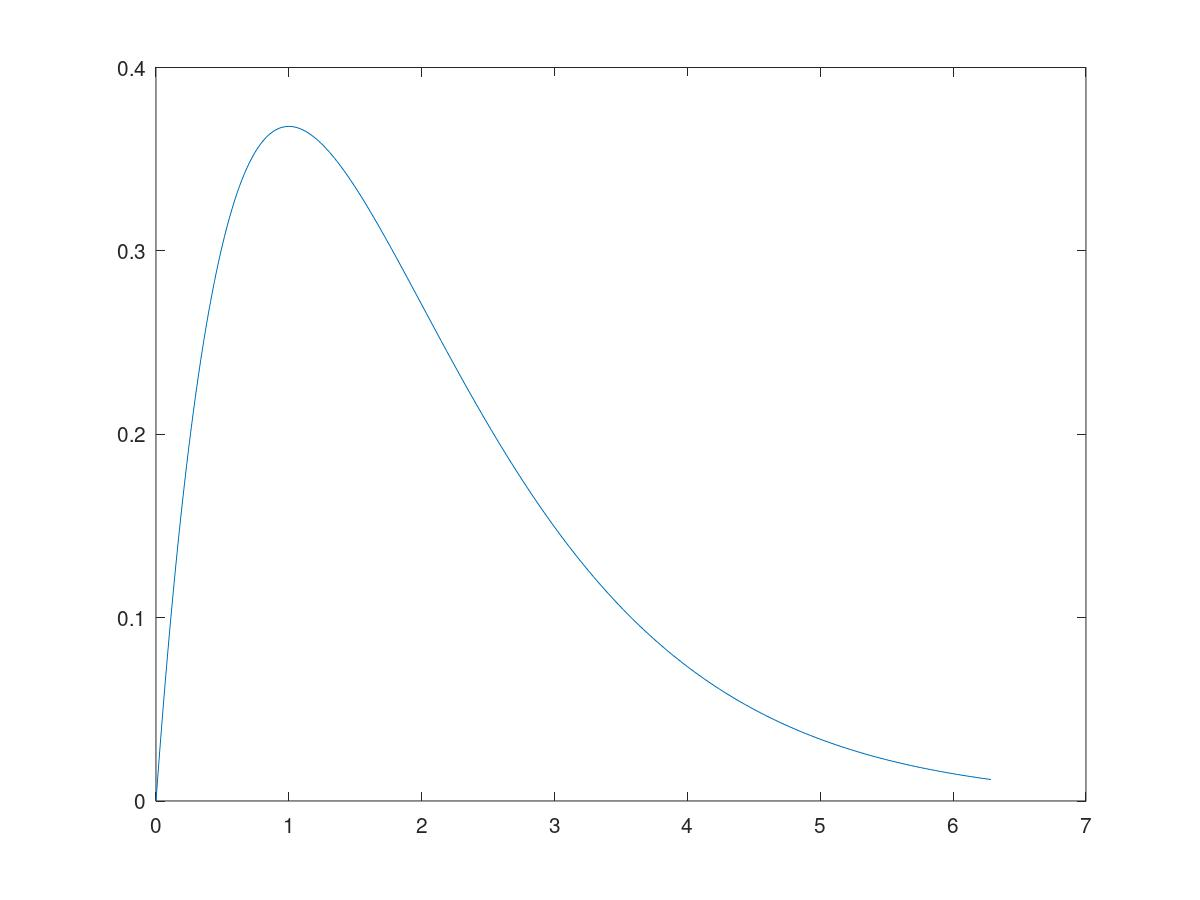
\includegraphics[width=\linewidth]{res/fig4.jpg}
        \caption{$f(x)$}
\end{figure}

\begin{lstlisting}[language=octave]
        octave:26> plot(x, y)
\end{lstlisting}

\begin{figure}[H]
        \centering
        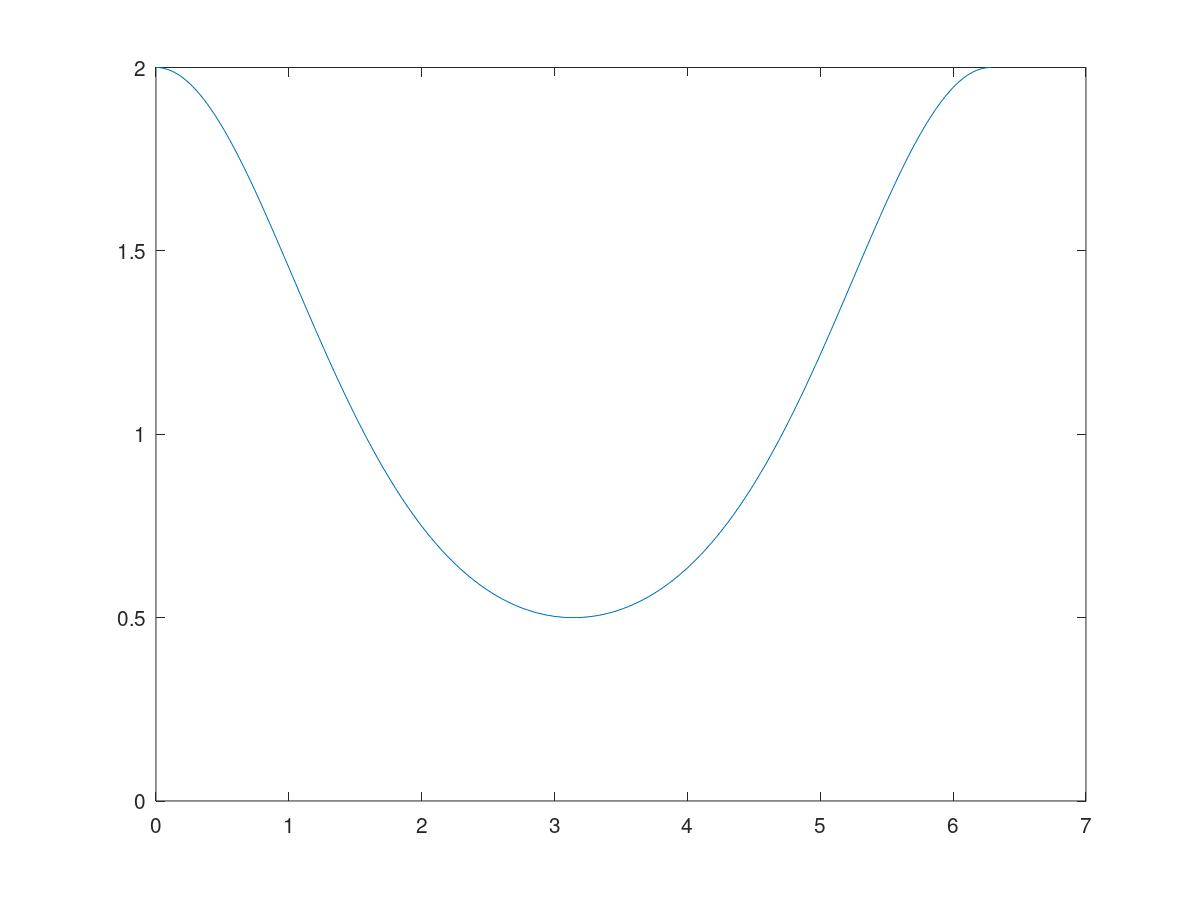
\includegraphics[width=\linewidth]{res/fig5.jpg}
        \caption{$f(x)$}
\end{figure}

\section{'Ασκηση 6}

\begin{itemize}
        \item Υπολογίστε τις μερικές παραγώγους της συνάρτησης:
                \[f(x, t) = \cos x + \sin t + e^t\]
        \item Υπολογίστε το ολοκλήρωμα:
                \[\int_{0}^{\infty} te^tdt\]
        \item Υπολογίστε το διπλό αόριστο ολοκλήρωμα:
                \[\iint x^3e^tdxdt\]
        \item Υπολογίστε το άθροισμα:
                \[\sum_{k = 0}^{\infty} \frac{x^k}{k!}\]
        \item Μετατρέψτε σε ρητή την παράσταση:
                \[f(x) = \frac{3}{x+2} + \frac{x}{x^2+1}\]
        \item Να λυθεί η εξίσωση δευτέρου βαθμού:
                \[f(x) = x^3 + 2x^2 - x - 2\]
\end{itemize}

Πρώτα από όλα, για την χρήση συναρτήσεων υπολογισμού παραγώγων και ολοκληρωμάτων,
χρειαζόμαστε το \lstinline{symbolic} πακέτο του Octave - κάτι αντίστοιχο υπάρχει
και στο Matlab. Αφού το εγκατασήσουμε, το φορτώνουμε στο Octave ως εξής:

\begin{lstlisting}[language=octave]
        octave:27> pkg load symbolic
\end{lstlisting}

\begin{itemize}
\item
Προκειμένου να υπολογίσουμε την μερική παράγωγο της συνάρτησης 
\[f(x, t) = \cos x + \sin t + e^t\]
πρέπει να ορίσουμε της συμβολικές μεταβλητές $x$ και $t$:
\begin{lstlisting}[language=octave]
        octave:28> syms x t
\end{lstlisting}

Στην συνέχεια ορίζουμε την συνάρτηση $f(x, t)$:
\begin{lstlisting}[language=octave]
        octave:29> y = cos(x) + sin(t) + e^t
        y = (sym)
\end{lstlisting}

Τέλος, υπολογίζουμε την μερική παράγωγο:

\[\frac{\partial}{\partial x}f(x, t) \Rightarrow
\frac{\partial}{\partial x}(\cos x + \sin t + e^t) \]

Για τον υπολογισμό της παραγώγου χρησιμοποιούμε την συνάρτηση
\lstinline{diff()}:
\begin{lstlisting}[language=octave]
        octave:30> diff(y, x)
        ans = (sym) -sin(x)
\end{lstlisting}

Μπορούμε να επαληθεύσουμε ότι το αποτέλεσμα είναι σωστό εφόσον:
\[\frac{\partial}{\partial x}(\cos x + \sin t + e^t) \Rightarrow
\frac{\partial}{\partial x} \cos x +
\frac{\partial}{\partial x} \sin t +
\frac{\partial}{\partial x} e^t \Rightarrow
-\sin x + 0 + 0 \Rightarrow -\sin x\]

\item
Για να υπολογίσουμε το ολοκλήρωμα
\[\int_{0}^{\infty} te^{-t}dt\]
αρχικά ορίζουμε την συνάρτηση που θέλουμε να ολοκληρώσουμε. Στο πρώτο
μέρος (\lstinline{@(t)}) ορίζουμε την μεταβλητή ως προς την οποία
θέλουμε να ολοκληρώσουμε:
\begin{lstlisting}[language=octave]
        octave:31> f = @(t) t *. e .^(-t)
\end{lstlisting}
Μετά με την χρήση της συνάρτησης \lstinline{integral()} υπολογίζουμε το
ολοκλήρωμα. Η συνάρτηση αυτή παίρνει τρία ορίσματα: την συνάρτηση, το πάνω
και το κάτω όριο. Οπότε:
\begin{lstlisting}[language=octave]
        octave:32> integral(f, 0, Inf)
        ans =  1
\end{lstlisting}

\item
Δεν υλοποιήθηκε λόγο απώλειας χρόνου.

\item
Δεν υλοποιήθηκε λόγο απώλειας χρόνου.

\item
Δεν υλοποιήθηκε λόγο απώλειας χρόνου.

\item
Για να λύσουμε την τριτοβάθμια εξίσωση:
\[f(x) = x^3 + 2x^2 - x - 2\]
oρίζουμε αρχικά την συμβολική μεταβλητή $x$ και την συνάρτηση $f(x)$:
\begin{lstlisting}[language=octave]
        octave:33> syms x
        octave:34> f = x^3 + 2*x^2 - x - 2
\end{lstlisting}
Βρίσκουμε τις ρίζες της παραπάνω τριτοβάθμιας εξίσωσης με την χρήση της
συνάρτησης \lstinline{solve()}:
\begin{lstlisting}[language=octave]
        octave:35> solve(f)
        ans = [-2 -1 1]
\end{lstlisting}

\end{itemize}

\section{'Ασκηση 7}

\begin{itemize}
        \item Να γραφεί function για τον υπολογισμό των ριζών ενός τριωνύμου.
\end{itemize}

Προκειμένου να υπολογίσουμε τις ρίζες ενός τριωνύμου χρειάζεται να χρησιμοποιήσουμε
λογικούς τελεστές και \lstinline{if} statements. Ο λόγος που χρειάζονται είναι
διότι υπάρχουνε ορισμένες περιπτώσεις που οι ρίζες του τριωνύμου δεν μπορούνε να
υπολογιστούν, και όταν μπορούν, μπορεί να έχουμε είτε μία είτε δύο ρίζες, οπότε
πρέπει να καλύψουμε όλες τις περιπτώσεις αυτές.

Ο τρόπος που δουλεύουνε τα \lstinline{if} statements στο Octave είναι ο ίδιος με
τις περισσότερες γλώσσες προγραμματισμού, δηλαδή:
\begin{lstlisting}[language=octave]
        if (condition)
                code
        elseif (condition)
                code
        else
                code
        endif
\end{lstlisting}

Αρχικά η συνάρτηση δέχεται τρία ορίσματα, τα $a$, $b$, και $c$ εφόσον το τριώνυμο
έχει την μορφή:
\[ax^2 + bx + c = 0\]

'Επειτα πρέπει να σιγουρέψουμε ότι το $a$ \textit{δεν} είναι 0, διότι σε αυτή την
περίπτωση δεν έχουμε δευτεροβάθμια εξίσωση.

Στην συνέχεια υπολογίζουμε την διακρίνουσα χρησιμοποιώντας τον κλασσικό τύπο:
\[d = b^2 - 4ac\]
και ελέγχουμε τις τιμές της.

Αν η διακρίνουσα είναι μεγαλύτερη του 0, τότε οι ρίζες είναι:
\[x_1, x_2 = \frac{-b \pm \sqrt d}{2a}\]

Αν η διακρίνουσα είναι ίση με 0, τότε έχουμε μία ρίζα:
\[x = \frac{-b}{2a}\]

Αν η διακρίνουσα είναι μικρότερη του 0 δεν έχουμε ρίζες.

Οπότε ο τελικός κώδικας που θα προκύψει είναι ο παρακάτω:

\begin{lstlisting}[language=octave]
        function quadratic(a, b, c)
                if (a != 0)
                        d = b^2 - 4*a*c
                        if (d > 0)
                                x1 = (-b + sqrt(d)) / (2 * a)
                                x2 = (-b - sqrt(d)) / (2 * a)
                        elseif (d == 0)
                                x = -b / (2 * a)
                        else
                                printf("no solutions\n")
                        endif
                else
                        printf("a cannot be 0\n")
                endif
        endfunction
\end{lstlisting}

Είναι καλύτερο να γράψουμε ένα αρχείο \lstinline{.m} που να
περιέχει τον παραπάνω κώδικα και να το τρέξουμε μέσα από
το Octave με την εντολή \lstinline{run()}. Αφού διαβαστεί το
αρχείο μπορούμε να καλέσουμε την συνάρτηση κανονικά, για
παράδειγμα:

\begin{lstlisting}[language=octave]
        octave:28> quadratic(2, 2, -4)
        d  =  36
        x1 =  1
        x2 = -2
\end{lstlisting}

\pagebreak
\section{Εργαλεία}
Τα εργαλεία που χρησιμοποιήθηκαν για την υλοποίηση αυτής της εργασίας ήτανε
τα εξής:

\begin{itemize}
        \item Περιβάλλον: GNU Octave 5.2.0
        \item Επιπλέον πακέτα: \lstinline{octave-forge-symbolic}
        \item Λειτουργικό σύστημα: FreeBSD 12.2
        \item Κειμενογράφος: Vim
        \item Μορφοποίηση κειμένου: \LaTeX
\end{itemize}
\end{document}
